\pagebreak
\section{Augmented Reality}

\subsection{Introduction}

This assignment has been divided to two main parts: drawing a cube and shading it. In the first part the emphasis was more on the mathematics behind the camera calibration, homographies and projections, whereas in the second part we have focused on calculating shading of the textured cube. similarly to the previous assignments, we used Python and OpenCV as a toolkit.

In the following text we describe the steps we took to complete the assignments. Each step is building on top of  the previous in a natural progression. We begin by describing how we used camera calibration to establish world coordinates, next we describe the steps necessary to project a wireframe cube into this world, followed by projecting a textured version of the cube, and backface culling to remove the faces not visible from the camera perspective.

In the second part of the assignment we enhance the textured cube from the first part by applying the Phong shading algorithm for a single light source


\subsection{Camera Calibration}
We started out by calibrating the camera using a chessboard pattern provided by the OpenCV library. This allowed us to compute both, intrinsic and extrinsic camera parameters as well as distortion coefficients for the camera. 

\begin{equation}
	P = K \begin{bmatrix} R|t \end{bmatrix}
\end{equation}

The intrinsic camera parameters \textit{K} do not change in time, because the camera we used does not have the ability to change the focal length of the lens, so it makes sense to store this data for later. 

The extrinsic parameters (\textit{R} and \textit{t}) on the other hand change with the position of the chessboard pattern.

Intrinsic and extrinsic parameters together make camera projection matrix \textit{P}. We use this matrix later to calculate homography between the first view we used to store the camera calibration and subsequent views in the rendering.

To verify that \textit{P} is correct we projected chess points on the first camera view. As you can see in the Figure \ref{subfig:chesspattern} all the points have been projected exactly into the right position.
 
 \begin{figure}[h!]
	\begin{subfigure}[b]{0.5\textwidth}
		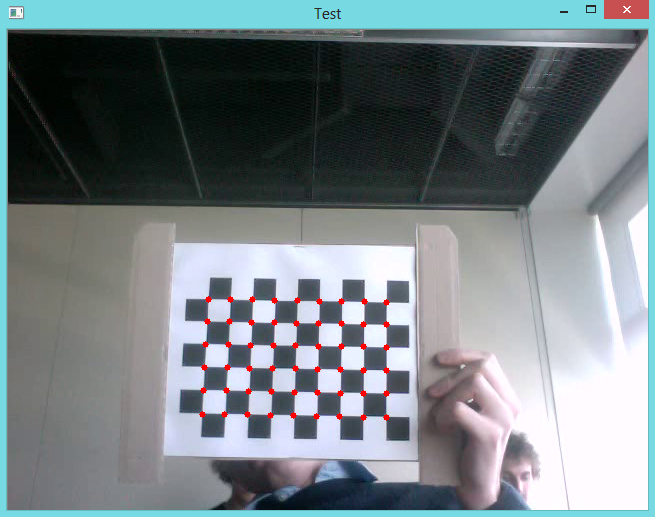
\includegraphics[width=\textwidth]{final/images/patterndot.jpg}
		\caption{Chessboard}
		\label{subfig:chesspattern}
	\end{subfigure}
	~
	\begin{subfigure}[b]{0.5\textwidth}
		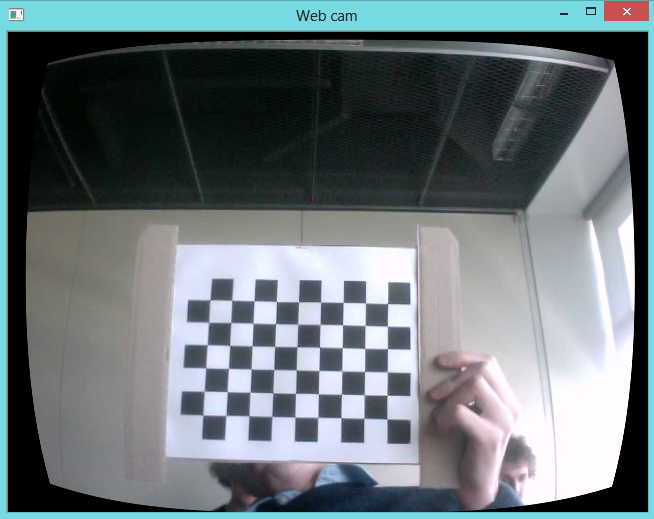
\includegraphics[width=\textwidth]{final/images/undistort.jpg}
		\caption{Undistort}
		\label{subfig:undistort}
	\end{subfigure}
	
	\caption{Camera Calibration}
\end{figure}
 
In the last step of this part we tried to undistort the image by using the (cv2.undistort) function. (see Figure \ref{subfig:undistort}). Using the chessboard, OpenCV has been able to calculate camera distortion coefficients, that we have stored for later use as well.

\subsection{Augmented Cube}
In this section, we calculated the full camera matrix in each frame and we used that for projecting a 3D cube into that frame. After that we tried to do the texture mapping on the faces of the cube we projected.

We tried two methods for calculating the projection camera. First method uses chessboard obtained from an arbitrary "first" image, and computes the homography between the first frame and the currently processed frame. It then uses the homography to construct the projection matrix for the camera. The second method uses just the chessboard pattern in the current frame to establish the world origin and relate the camera position towards it.

The second method gives us a better result, because the first method computes the homography between two frames and because the frames can have relative distortion with each other and an absolute distortion it will slightly worse result.

Now that we found the camera matrix with both methods for testing them we tried to project the chesspattern points in the world coordinate system to the current camera view. All points were projected to the right place in the image so we moved to the next step.

In this step we drew the world coordinate axes attached to the chesspattern plane and then we projected the cube into the current view again attached to the pattern plane. In order to do this, we had a representation of the cube in object coordinates, and we have positioned it in the world without any translation, rotation or scaling. Thanks to this, it was possible for us to treat the coordinates of the cube object coordinate system as if they were in the world coordinate system. Otherwise we would have to transform them from object coordinate system into world coordinate system.

 \begin{figure}[h!]
	\centering
	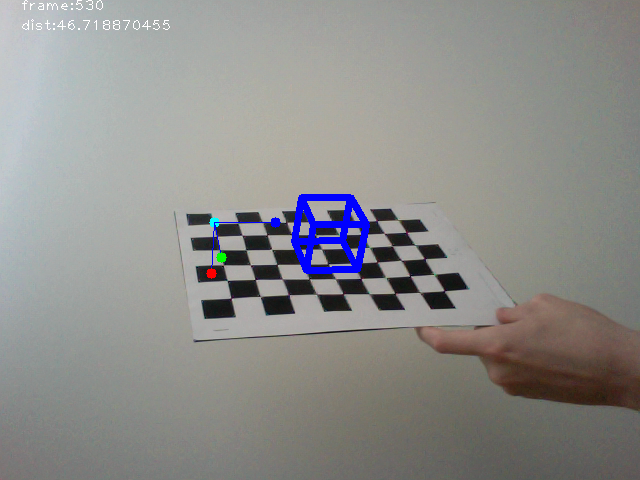
\includegraphics[width=\textwidth]{final/images/wireframe.png}
	\caption{Wireframe Cube}
	\label{fig:wireframe}
\end{figure}

To draw a wireframe model in Figure \ref{fig:wireframe} we simply take a pair of points from the cube that form an edge, project them using the projection matrix we calculated before to obtain their positions in the 2D image and then just draw a line between them.

\subsection{Back-face Culling and Texture Mapping}

To texture our wireframe model, we first calculate the homography between the texture (2D image) and a face of the cube as it is projected in the 2D final image. We then use this homography to perspective warp the texture into the final image. See Figure \ref{subfig:texture}. But this is obviously not right, some faces overlap others randomly. We solve this by a technique called back-face culling.

Back-face culling is a technique we have employed to address the problem that appears when we render the whole cube. In the 2D view you can not see all 5 textured faces of the cube at once. It is only possible to see one to three faces at any given time. Therefore some faces we render are redundant. All faces are drawn in the order in which the list containing their names is processed, so it is the same order always. Therefore the faces that are drawn later occlude faces drawn earlier, even though logically they should be behind them. 

To address this problem, a simple technique has been developed, where we determine the angle between the camera and a face, and based on that we decide whether or not to show the face. First we compute the unitary normal vector of the face. We take three points from the face, since we assume that the face is composed of four coplanar points, it does not matter which three we take, but the order does matter, because with wrong order we will get a normal that faces the other way (inside the cube). We then construct displacement vectors between two point pairs of the three points, and calculate the cross product of these vectors. As the last step we transform the obtained vector to get a unitary vector. 

Similarly we compute a vector from camera center and the center of the face we are comparing. We transform this vector to unitary as well. We can calculate the angle between the two vectors. If this angle is greater than 90 degrees, we know that the face is facing away from the camera, and we therefore do not draw it.

 \begin{figure}[h!]
	\begin{subfigure}[b]{0.5\textwidth}
		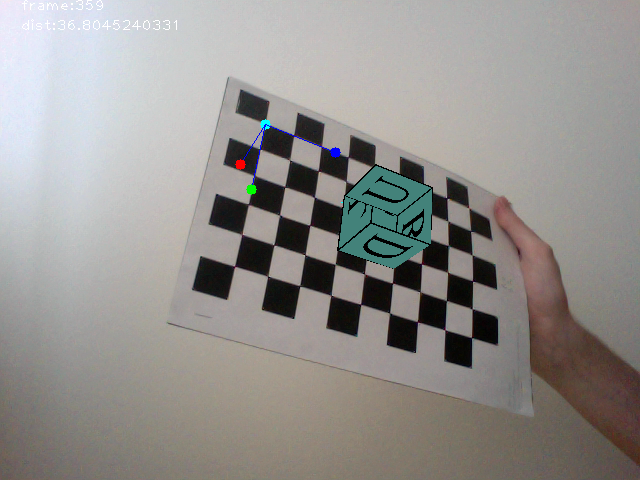
\includegraphics[width=\textwidth]{final/images/culling.png}
		\caption{Texture Mapping}
		\label{subfig:texture}
	\end{subfigure}
	~
	\begin{subfigure}[b]{0.5\textwidth}
		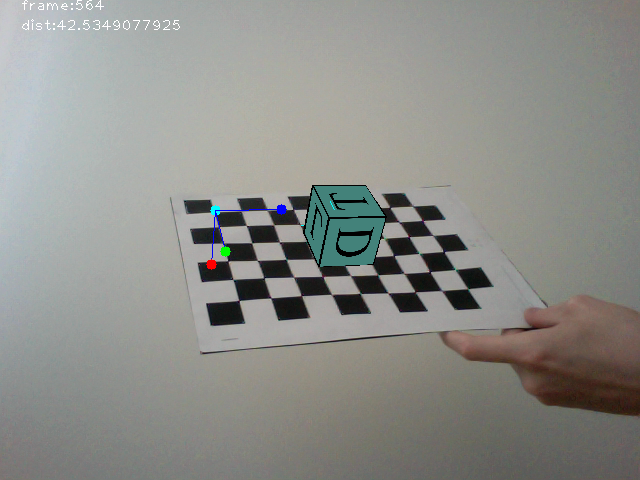
\includegraphics[width=\textwidth]{final/images/texture2.png}
		\caption{Back-face Culling}
		\label{subfig:backculling}
	\end{subfigure}
	
	\label{fig:texturing}
	\caption{Backface Culling and Texture Mapping}
\end{figure}

\subsection{Shading}

Shading is a process that is often applied to 3D rendered objects to make them appear more realistic by modeling  how light interacts with them. In the code we have implemented, we have used the Equation \ref{eq:shading}. In the equation \textit{I} is final illuminated texture of a face, \textit{T(u, v)} is the texture of the face with dimensions s and t. \textit{L\textsubscript{a}} is the ambient illumination, \textit{k\textsubscript{a}} is the ambient component of the object's material. \textit{L\textsubscript{l}} is light intensity, \textit{k\textsubscript{d}} is the diffuse component of the material. \textit{n} is the face normal vector. \textit{k\textsubscript{s}} is the specular component of the material. \textit{v} is the viewer vector and \textit{r\textsubscript{i}} is the reflected light vector. All vectors are unitary.

\begin{equation}
	I=T(u,v)[
	\underbrace{
	L_{a}k_{a}
	}_\text{Ambient}
	+
	\underbrace{
	k_{d}\sum\limits_{i}L_{i}max(n\cdot l_{i},0)
	}_\text{Diffuse}
	+
	\underbrace{
	k_{s}\sum\limits_{i}L_{i}(r_{i}\cdot v)^\alpha
	  }_\text{Specular}
	]
	\label{eq:shading}
\end{equation}

This equation differs slightly from what has been implemented in our report, because it allows for multiple light sources, whereas we have only implemented one light source. On the other hand both the equation, and our implementation assume the material is uniform, while it could easily be a texture.

To shade the individual faces in our project, we used a low resolution (10$\times$10) texture that we have multiplied with the texture calculated from before. We have implemented two different approaches to shading, the flat shading model and and Phong shading model. In both models, the underlying equation is the same (Figure \ref{eq:shading}), but there are differences in how it is applied.

In the flat shading model, we only need to calculate one diffuse and specular value per face, and apply it to the whole face.

In contrast, Phong shading model assigns each pixel in our light texture a different normal, calculated using bilinear interpolation from corner normals of the currently evaluated face. The corner normals are calculated by averaging the normals of all neighboring faces. The result of all of this is that there is a smooth transition between normals calculated for points along the face. This allows us to draw objects with relatively small face counts (and therefore smaller and easier to store and manipulate) easily and with nice smooth surface. 

This means that we can then use this normal to calculate the illumination at a single point of the face texture to obtain a smooth gradient corresponding to diffuse and specular light. 

All that remains is then to combine the illumination texture with the original texture to shade the face and project it to create the final image. Of course this is repeated for every face.

We have also implemented different light positions. It is possible to click into the camera window and select a new position for the light, which is by default positioned in the camera center, see Figure \ref{subfig:extra1} and \ref{subfig:extra2}. 

 \begin{figure}[h!]
	\begin{subfigure}[b]{0.5\textwidth}
		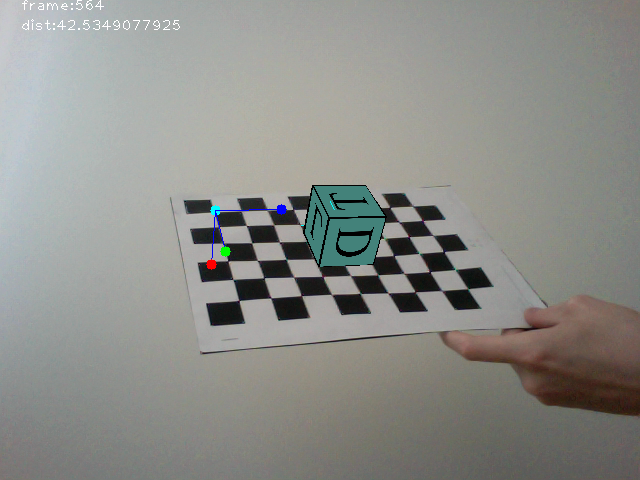
\includegraphics[width=\textwidth]{final/images/texture2.png}
		\caption{Plain Texture Mapping}
		\label{subfig:plaintexture}
	\end{subfigure}
	~
	\begin{subfigure}[b]{0.5\textwidth}
		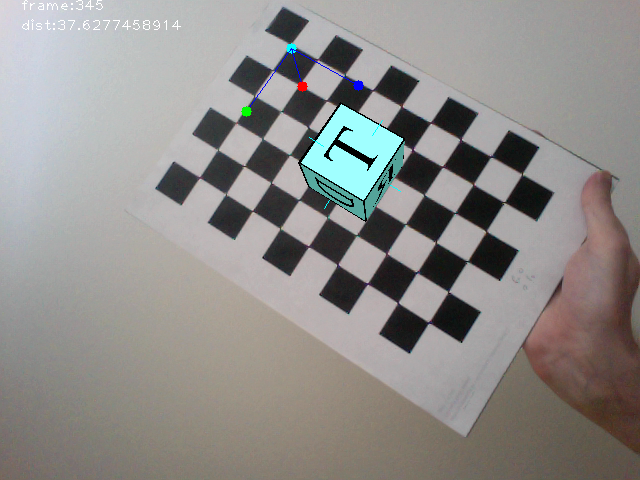
\includegraphics[width=\textwidth]{final/images/flat.png}
		\caption{Flat Shading}
		\label{subfig:flatshading}
	\end{subfigure}
	~
	\begin{subfigure}[b]{0.5\textwidth}
		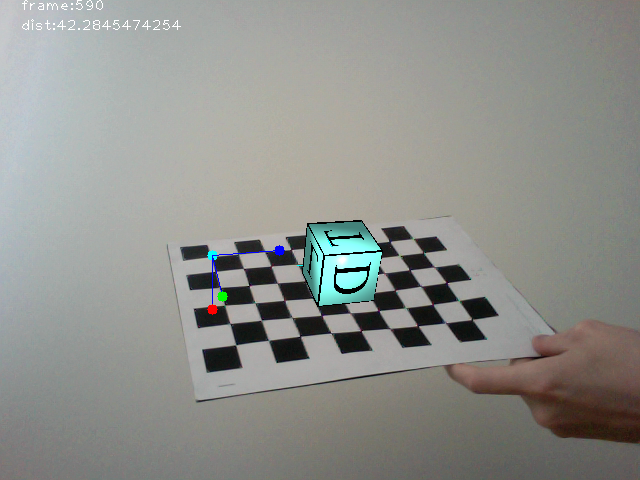
\includegraphics[width=\textwidth]{final/images/phong1.png}
		\caption{Phong Shading}
		\label{subfig:phongshading}
	\end{subfigure}
	~
	\begin{subfigure}[b]{0.5\textwidth}
		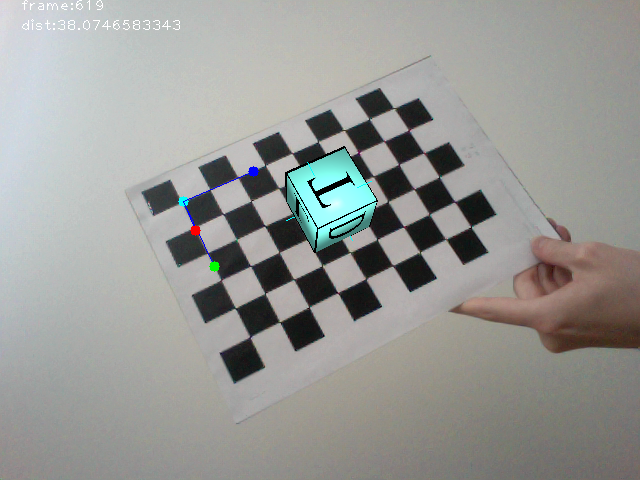
\includegraphics[width=\textwidth]{final/images/phong2.png}
		\caption{Phong Shading 2}
		\label{subfig:phongshading2}
	\end{subfigure}
\end{figure}
 \begin{figure}[h!]
	\begin{subfigure}[b]{0.5\textwidth}
		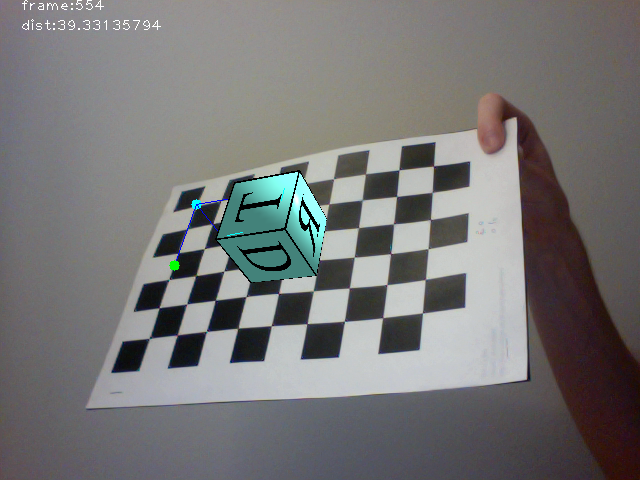
\includegraphics[width=\textwidth]{final/images/extra1.png}
		\caption{Light Position Top Right}
		\label{subfig:extra1}
	\end{subfigure}
	~
	\begin{subfigure}[b]{0.5\textwidth}
		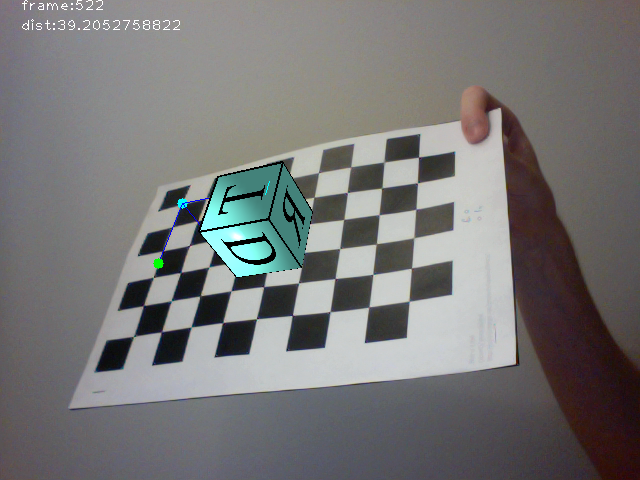
\includegraphics[width=\textwidth]{final/images/extra2.png}
		\caption{Light Position Bottom Left}
		\label{subfig:extra2}
	\end{subfigure}
	
	\label{fig:texturing}
	\caption{Shading}
\end{figure}

\subsection{Conclusion}

In this assignment we have worked with various techniques that are in use in the field of computer graphics. We have looked at how homographies are useful in calculating camera projection matrices and how those matrices are useful in projecting 3D world onto a 2D image. We have tried out texturing a 3D object and we have explored the intricate mathematics of shading models. We found it very useful and applicable in many areas, such as augmented reality, 3D programming, etc. In the end we have been successful in implementing all the methods and techniques described, and we have deepened our knowledge of the 3D concepts in use.


